% ============================================================
%  Sprawozdanie: Badanie polaryzacji światła (POLAR)
%  Fotonika – laboratorium, ZUT Szczecin
% ============================================================
\documentclass[a4paper,12pt]{article}

\usepackage[utf8]{inputenc}
\usepackage[T1]{fontenc}
\usepackage{lmodern}
\usepackage[polish]{babel}
\usepackage{geometry}
\geometry{a4paper, top=2.2cm, bottom=2.2cm, left=2.5cm, right=2.5cm}

\usepackage{amsmath,amssymb}
\usepackage{booktabs}
\usepackage{graphicx}
\usepackage{float}
\usepackage{caption}
\usepackage{multirow}
\usepackage{array}
\usepackage{xcolor}
\usepackage{hyperref}
\usepackage{siunitx}
\sisetup{output-decimal-marker={,}, locale=DE}
\usepackage{parskip}
\setlength{\parskip}{4pt}

\graphicspath{{../}}

\title{}
\date{}

\begin{document}

% ============================================================
%  TABELA NAGŁÓWKOWA (punkty 1–3)
% ============================================================
\begin{table}[H]
\centering
\small
\renewcommand{\arraystretch}{1.3}
\resizebox{\textwidth}{!}{%
\begin{tabular}{|*{12}{c|}}
\hline
\multicolumn{12}{|c|}{\textbf{Zachodniopomorski Uniwersytet Technologiczny w Szczecinie}} \\
\hline
\multicolumn{2}{|c|}{Przedmiot:} & \multicolumn{10}{c|}{Fotonika} \\
\hline
\multicolumn{2}{|c|}{Prowadzący:} & \multicolumn{10}{c|}{Mgr. Inż. Eliza Miśkiewicz} \\
\hline
\multicolumn{12}{|c|}{\textbf{SPRAWOZDANIE Z WYKONANEGO ĆWICZENIA}} \\
\hline
\multicolumn{2}{|c|}{Nr ćw.: 4} & 02 & \multicolumn{2}{c|}{Temat:} & \multicolumn{7}{c|}{POLARYZACJA (POLAR)} \\
\hline
Zespół lab.: & 5 & Grupa: & L1 & Studia: & S2 & Kierunek: & TI & Rok: & 2025/2026 & Data: & 30.03.2026 \\
\hline
\multicolumn{3}{|c|}{Skład zespołu wg. obecności podczas ćwiczenia:} & \multicolumn{9}{c|}{1. Piotr Gadomski} \\
\hline
\multicolumn{2}{|c|}{Ocena:} & \multicolumn{10}{c|}{} \\
\hline
\end{tabular}%
}
\end{table}

% ============================================================
\section*{Cel ćwiczenia}
% ============================================================

Celem ćwiczenia było poznanie zjawiska polaryzacji światła, doświadczalne wyznaczenie
kąta Brewstera dla płytki kwarcowej, obliczenie jej współczynnika załamania $n$ oraz
zbadanie skuteczności stosu polaryzacyjnego (15 płytek szklanych) jako polaryzatora
liniowego.

% ============================================================
\section*{Wstęp teoretyczny}
% ============================================================

Światło jako fala elektromagnetyczna charakteryzuje się poprzecznym kierunkiem drgań
wektora pola elektrycznego $\mathbf{E}$. W świetle niespolaryzowanym kierunek ten
zmienia się chaotycznie, natomiast w świetle spolaryzowanym liniowo wektor $\mathbf{E}$
drga w jednej, ściśle określonej płaszczyźnie.

\textbf{Prawo Malusa} opisuje natężenie światła spolaryzowanego liniowo po przejściu
przez analizator (drugi polaryzator) ustawiony pod kątem $\varphi$ do płaszczyzny
polaryzacji:
\[
I = I_0 \cos^2\varphi .
\]

\textbf{Kąt Brewstera.} Gdy niespolaryzowana wiązka światła pada na granicę dwóch
ośrodków dielektrycznych pod pewnym kątem $\theta_B$ (kąt Brewstera), wiązka odbita
staje się całkowicie spolaryzowana liniowo — zawiera wyłącznie składową s (wektor
$\mathbf{E}$ prostopadły do płaszczyzny padania). Dla kąta Brewstera spełniona jest
zależność:
\[
n = \tan\theta_B ,
\]
gdzie $n = n_2/n_1$ jest względnym współczynnikiem załamania. Dla granicy powietrze--dielektryk
($n_1 \approx 1$) otrzymujemy $n \approx \tan\theta_B$.

\textbf{Stos polaryzacyjny} zbudowany z wielu ($N$) płytek szklanych ustawionych pod
kątem Brewstera pozwala uzyskać wysoki stopień polaryzacji wiązki przechodzącej. Przy
każdym odbiciu usuwana jest część składowej s, podczas gdy składowa p przechodzi bez
odbicia ($r_p = 0$). Po przejściu przez $N$ płytek wiązka przepuszczona jest prawie
w pełni spolaryzowana poziomo (polaryzacja p).

Stopień polaryzacji wyznacza się ze wzoru:
\[
P = \frac{I_{\max} - I_{\min}}{I_{\max} + I_{\min}} .
\]

% ============================================================
\section*{Schematy układów pomiarowych}
% ============================================================

\begin{figure}[H]
\centering
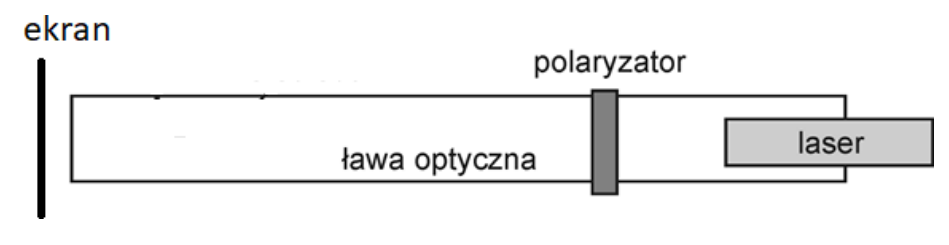
\includegraphics[width=0.85\textwidth]{Rys1.png}
\caption{Układ do analizy stanu polaryzacji światła generowanego przez laser
(Laser He-Ne, P -- polaryzator obrotowy, E -- ekran/detektor).}
\end{figure}

\begin{figure}[H]
\centering
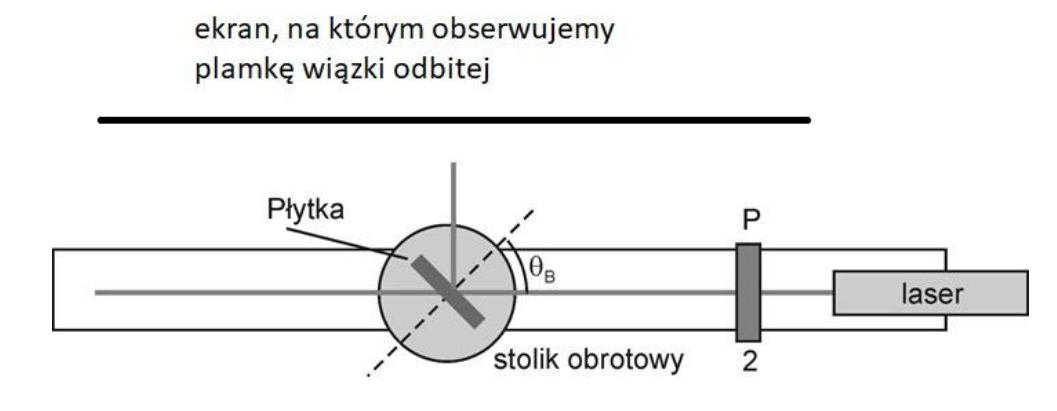
\includegraphics[width=0.85\textwidth]{Rys2.png}
\caption{Układ do wyznaczenia kąta Brewstera. P -- polaryzator z poziomą osią
transmisji, płytka kwarcowa na stoliku obrotowym, E -- ekran, FD -- fotodetektor.}
\end{figure}

% ============================================================
\section*{Spis przyrządów pomiarowych}
% ============================================================

\begin{itemize}
  \item Laser He-Ne (helowo-neonowy, $\lambda = \SI{632,8}{nm}$) firmy Spectra Physics z zasilaczem.
  \item Obrotowy polaryzator liniowy (polaryzator P / analizator A).
  \item Płytka kwarcowa na stoliku obrotowym ze skalą kątową (działka $\Delta\alpha = \SI{1}{\degree}$).
  \item Stos polaryzacyjny (15 szkiełek mikroskopowych).
  \item Fotodetektor (FD) z miernikiem mocy optycznej (zakres do ok. \SI{15}{mW}).
  \item Ława optyczna i ekran.
\end{itemize}

% ============================================================
\section*{Przebieg ćwiczenia}
% ============================================================

\textbf{Część A -- Badanie polaryzacji światła lasera.}
\begin{enumerate}
  \item Zestawiono układ: Laser $\to$ Polaryzator P $\to$ Ekran/detektor.
  \item Obracając polaryzator P o pełny obrót obserwowano plamkę na ekranie i wskazania
  miernika mocy.
  \item Stwierdzono, że natężenie wiązki zmienia się i przy pewnym ustawieniu polaryzatora
  ulega całkowitemu wygaszeniu -- świadczy to o liniowej polaryzacji światła lasera He-Ne.
\end{enumerate}

\textbf{Część B -- Wyznaczenie kąta Brewstera dla płytki kwarcowej.}
\begin{enumerate}
  \item Zestawiono układ: Laser $\to$ Polaryzator P (oś pozioma) $\to$ Płytka kwarcowa
  na stoliku $\to$ Ekran/FD.
  \item Ustawiono polaryzator P tak, aby oś transmisji była pozioma (polaryzacja p).
  \item Pokryto kreski zerowe na skalach stolika, ustawiono płytkę prostopadle do wiązki.
  \item Odblokowano stolik i obracano go do momentu zaniku wiązki odbitej na ekranie.
  \item Odczytywano kąt obrotu $\theta_B$ na skali stolika. Pomiar powtórzono 5-krotnie,
  za każdym razem wracając do pozycji zerowej.
  \item Obliczono wartość średnią $\bar{\theta}_B$ i niepewności pomiarowe.
  \item Wyznaczono współczynnik załamania $n = \tan\bar{\theta}_B$ wraz z niepewnością
  metodą różniczki zupełnej.
\end{enumerate}

\textbf{Część C -- Badanie stosu polaryzacyjnego.}
\begin{enumerate}
  \item W miejsce płytki kwarcowej wstawiono stos 15 płytek szklanych, ustawiony
  pod wyznaczonym kątem Brewstera.
  \item Za stosem umieszczono analizator A i fotodetektor FD.
  \item Obracając analizator zarejestrowano maksymalną i minimalną moc optyczną
  wiązki przechodzącej.
  \item Obliczono stopień polaryzacji $P$ i dynamikę polaryzatora $\eta$ w decybelach.
\end{enumerate}

% ============================================================
\section*{Wyniki pomiarów i obliczenia}
% ============================================================

\subsection*{1. Wyznaczanie współczynnika załamania płytki kwarcowej}

Wyniki pięciu pomiarów kąta Brewstera $\theta_B$:
\[
\theta_{B,1} = 56^\circ,\quad
\theta_{B,2} = 56^\circ,\quad
\theta_{B,3} = 56^\circ,\quad
\theta_{B,4} = 56^\circ,\quad
\theta_{B,5} = 56^\circ.
\]

Wartość średnia:
\[
\bar{\theta}_B = \frac{1}{5}\sum_{i=1}^{5}\theta_{B,i} = \SI{56,0}{\degree}.
\]

\textbf{Niepewność typu A} (przypadkowa) -- odchylenie standardowe średniej:
\[
s(\theta_B) = \sqrt{\frac{\sum(\theta_{B,i}-\bar{\theta}_B)^2}{N-1}} = 0,\qquad
u_A(\theta_B) = \frac{s(\theta_B)}{\sqrt{N}} = \SI{0,000}{\degree}.
\]
Wszystkie pomiary dały identyczny wynik, stąd $u_A = 0$.

\textbf{Niepewność typu B} (systematyczna) -- związana z działką elementarną skali
stolika $\Delta\alpha = \SI{1}{\degree}$:
\[
\Delta\alpha = \SI{1}{\degree} = \SI{0,01745}{rad},\qquad
u_B(\alpha) = \frac{\Delta\alpha}{\sqrt{3}} = \frac{\SI{0,01745}{rad}}{\sqrt{3}}
= \SI{0,01008}{rad}.
\]

\textbf{Niepewność całkowita} kąta:
\[
u(\alpha) = \sqrt{u_A^2 + u_B^2} = \sqrt{0^2 + 0{,}01008^2} = \SI{0,01008}{rad}.
\]

\textbf{Współczynnik załamania} płytki:
\[
n = \tan\bar{\theta}_B = \tan(56{,}0^\circ) = 1{,}4826.
\]

\textbf{Niepewność $u(n)$} metodą różniczki zupełnej:
\[
u(n) = \left|\frac{dn}{d\alpha}\right| u(\alpha)
= \frac{1}{\cos^2\bar{\theta}_B}\,u(\alpha)
= \frac{1}{\cos^2(56{,}0^\circ)} \cdot 0{,}01008
= 3{,}198 \cdot 0{,}01008 = 0{,}03223.
\]

\textbf{Niepewność rozszerzona} (dla $K = 2$, poziom ufności ok. 95\%):
\[
U(n) = K \cdot u(n) = 2 \cdot 0{,}03223 = 0{,}06445.
\]

\textbf{Wynik końcowy:}
\[
\boxed{n = 1{,}483 \pm 0{,}064}.
\]

\begin{table}[H]
\centering
\caption{Niepewności systematyczne i przypadkowe -- podsumowanie.}
\renewcommand{\arraystretch}{1.3}
\small
\begin{tabular}{c S[table-format=2.1] S[table-format=1.4] S[table-format=1.5] S[table-format=1.5] S[table-format=1.5] S[table-format=1.4] S[table-format=1.5] S[table-format=1.5]}
\toprule
{$\alpha$} & {$\bar{\alpha}$ [\si{\degree}]} & {$u_A(\alpha)$ [\si{\degree}]} & {$\Delta\alpha$ [rad]} & {$u_B(\alpha)$ [rad]} & {$u(\alpha)$ [rad]} & {$n$} & {$u(n)$} & {$U(n)$} \\
\midrule
5$\times$56 & 56,0 & 0,0000 & 0,01745 & 0,01008 & 0,01008 & 1,4826 & 0,03223 & 0,06445 \\
\bottomrule
\end{tabular}
\end{table}

\subsection*{2. Badanie stosu polaryzacyjnego}

Wyniki pomiaru mocy optycznej wiązki przechodzącej przez stos 15 płytek:

\begin{table}[H]
\centering
\caption{Stos płytek szklanych jako polaryzator.}
\renewcommand{\arraystretch}{1.3}
\begin{tabular}{cc}
\toprule
Polaryzacja pionowa wiązki & Polaryzacja pozioma wiązki \\
\midrule
\multicolumn{2}{c}{Pomiar natężenia światła miernikiem} \\
\midrule
$P_{\text{pion}} = \SI{0,03}{mW}$ & $P_{\text{poz}} = \SI{0,34}{mW}$ \\
\bottomrule
\end{tabular}
\end{table}

\textbf{Dynamika polaryzatora:}
\[
\eta = \frac{P_{\max}}{P_{\min}} = \frac{0{,}34}{0{,}03} = 11{,}33,
\]
\[
\eta_{\text{dB}} = 10\log_{10}(\eta) = 10\log_{10}(11{,}33) = \SI{10,54}{dB}.
\]

\textbf{Stopień polaryzacji:}
\[
P = \frac{I_{\max} - I_{\min}}{I_{\max} + I_{\min}}
= \frac{0{,}34 - 0{,}03}{0{,}34 + 0{,}03}
= \frac{0{,}31}{0{,}37} = 0{,}838.
\]

Wiązka przechodząca przez stos ma dominującą składową poziomą (polaryzacja p), co jest
zgodne z teorią -- składowa pionowa (s) jest stopniowo usuwana przy kolejnych odbiciach
od płytek ustawionych pod kątem Brewstera.

% ============================================================
\section*{Wnioski}
% ============================================================

\begin{enumerate}
  \item Światło lasera He-Ne jest spolaryzowane liniowo -- przy obrocie polaryzatora
  zaobserwowano całkowite wygaszenie wiązki, zgodnie z prawem Malusa.

  \item Wyznaczony kąt Brewstera dla płytki kwarcowej wynosi $\bar{\theta}_B = \SI{56,0}{\degree}$.
  Ponieważ wszystkie 5 pomiarów dało identyczną wartość, niepewność typu A wynosi zero,
  a o~niepewności całkowitej decyduje niepewność systematyczna skali stolika ($\Delta\alpha = 1^\circ$).

  \item Współczynnik załamania płytki wyznaczony z zależności $n = \tan\theta_B$ wynosi:
  \[
  n = 1{,}483 \pm 0{,}064 .
  \]
  Otrzymana wartość jest zbliżona do wartości $n \approx 1{,}47$ dla szkła kwarcowego
  przy $\lambda \approx \SI{0,6}{\mu m}$ (laser He-Ne). Sugeruje to, że badana płytka
  wykonana jest ze szkła kwarcowego, a nie z kwarcu krystalicznego ($n \approx 1{,}54$).

  \item Stos 15 płytek szklanych działa jako skuteczny polaryzator liniowy. Dynamika
  polaryzatora wynosi $\eta = \SI{10,54}{dB}$, a stopień polaryzacji $P = 0{,}838$.
  Wiązka przepuszczona jest spolaryzowana poziomo (polaryzacja p) -- analizator
  wskazuje minimum przy orientacji pionowej ($P_{\text{pion}} = \SI{0,03}{mW}$),
  a~maksimum przy orientacji poziomej ($P_{\text{poz}} = \SI{0,34}{mW}$).

  \item Uzyskany stopień polaryzacji ($P = 0{,}838$) jest niższy od wartości teoretycznej
  dla 15 płytek ($P \approx 0{,}985$). Przyczyną może być niedokładne ustawienie kąta
  Brewstera, niedoskonałości powierzchni szkiełek mikroskopowych oraz wpływ światła
  otoczenia na pomiar fotodetektorem.
\end{enumerate}

\end{document}
